\chapter{Relevant Background}
\label{cha:chapter3}

\section{Neural Networks}
Neural networks (NNs) are a type of machine learning algorithms that are inspired by how human brain works.  In particular, a NN has units called neurons connected to each other similar to the way neurons in the human brain are. The connections between neurons allow the NN to build hierarchical representations that are necessary to perform an objective task. \addfigure{\ref{fig:nn_typical_structure}} illustrates the basic structure of a NN. The network has an input layer, output layer, and hidden layers. The figure also shows connections of neurons connecting to other neurons in neighbor layers. 

Given an objective task, the goal is to construct connections between these neurons such that the network can transform an input sample into the desired output.  These connections are determined by trainable weights and biases, denoted as $w_{ij}, w_{jk}$ and $b_j$ respectively in the figure, where $w_{ij}$ refers to a weight between a neuron $i$ to a neuron $j$ in the following layer.

%\addfigure{\ref{fig:nn_simple}} illustrates a reaction task that neurons in our brain perform together to achieve. 

%todo supervise vs unsupervise
%
% \begin{figure}[ht!]
%    \begin{center}
%
%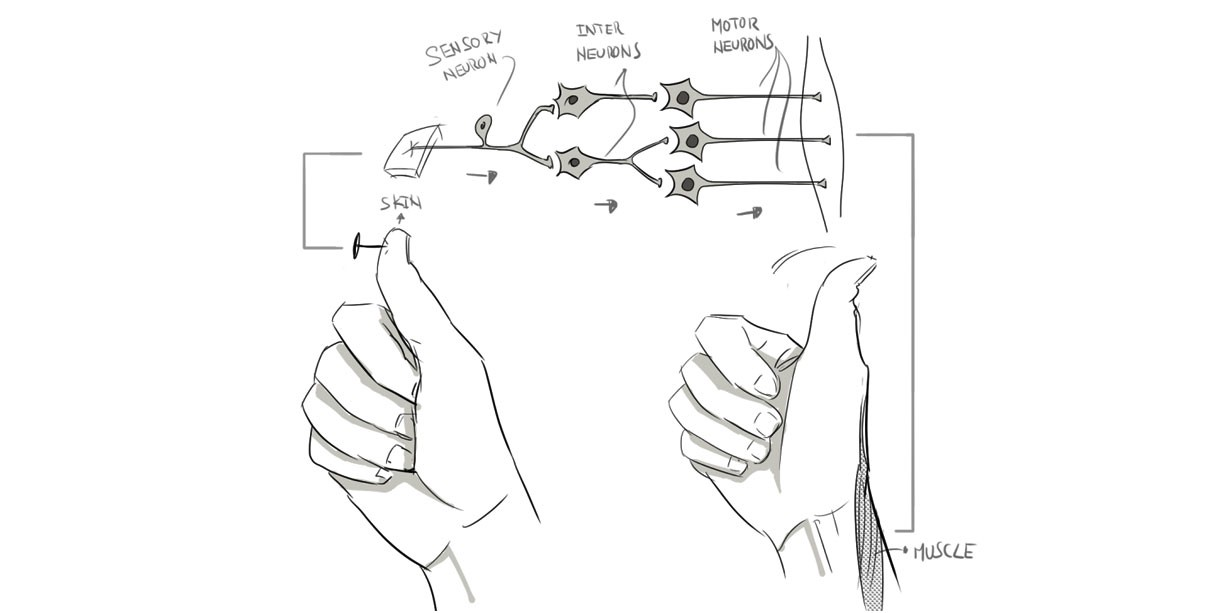
\includegraphics[width=\textwidth]{nn_simple}
%\caption{An illustration of how neurons in the human brain interact to sense the pain and react accordingly.}
%\small{Source : \cite{LeonMakingSimpleNeural2017}}
%% todo change this figure
%\label{fig:nn_simple}
%
%\end{center}
%\end{figure}

 \begin{figure}
    \begin{center}

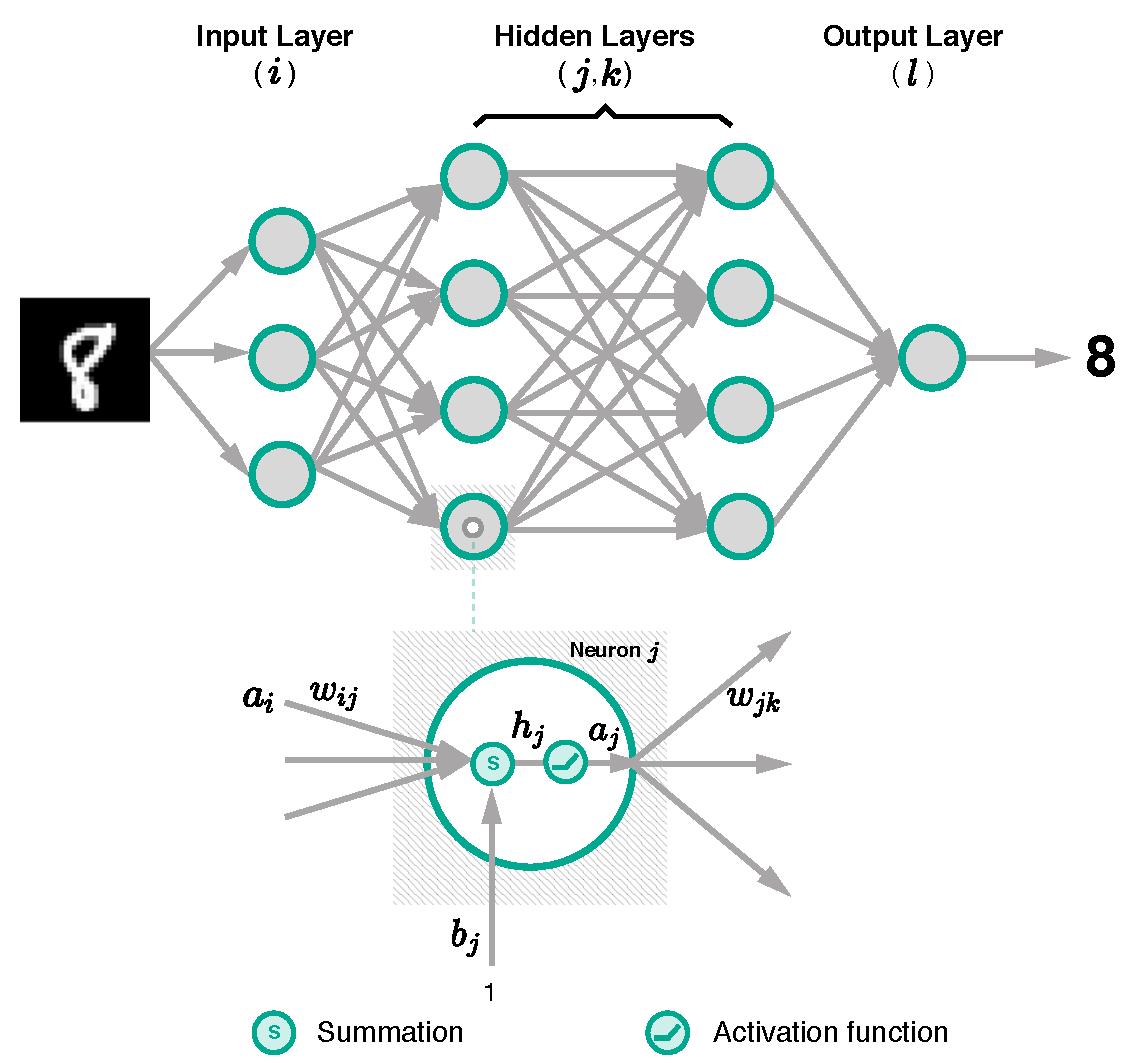
\includegraphics[width=0.8\textwidth]{sketch/typical_nn_structure}
%\caption[]{Basic structure of a neural network. between neurons.}
\patcaption{Basic structure of a neural network.}{}
\label{fig:nn_typical_structure}

\end{center}
\end{figure}


% \begin{figure}[ht!]
%	\begin{center}
%
%		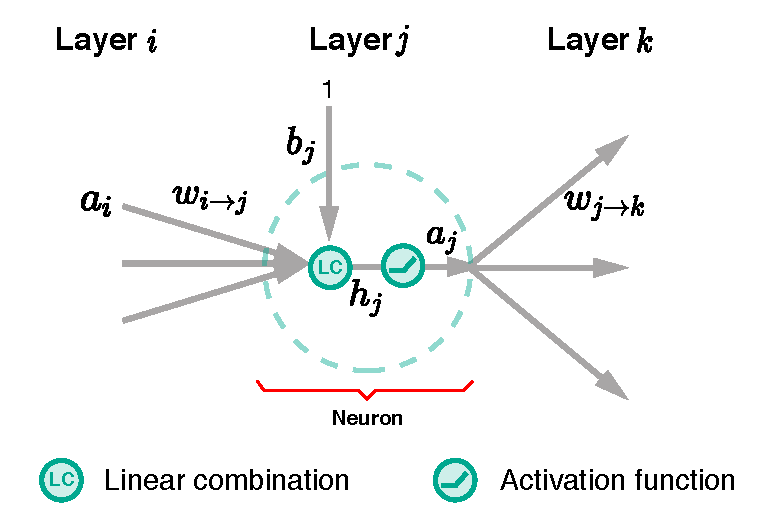
\includegraphics[width=0.5\textwidth]{sketch/a_neuron}
%		\caption{Connectivity and activity of a neuron}
%		\label{fig:a_neuron}
%	\end{center}
%\end{figure}




 Mathematically, a NN can be viewed as a function $f$ with parameters $\patvector{\theta} = \{\forall i,j,k : w_{ij}, w_{jk}, w_{kl}, b_j, b_k, b_l \}$  non-linearly transforming an input $\x \in \mathbb{R}^d $ to some output $f(\x)$. For supervised tasks, such as classification or regression, we hope that $f(\x)$ will be close to the true label $y$.
%
%Consider a given set of $p$ training samples $\mathcal{D} = \{ \xa, \ya) \}_{\alpha=1}^{p}$,  there are 3 primary components to build a NN, namely  
%
%More formally, when referring to a NN, we associate it to a certain architecture that describes settings of the network. Such settings are number of layers, number of neurons in each layer and type of activation function.  Typically, the weights and biases are denoted as $\patvector{\theta}$. Mathematically, NN can be viewed as a function $f$ with parameters $\patvector{\theta}$ that nonlinearly transforms an input $\xa\in \mathbb{R}^d $ to some output $f(\xa)$.
%
%These variables will be learned  during \textit{training} process. 



\subsection{Loss functions}
A \textit{loss function} $L$  is a measurement that quantifies whether the predicted output $f(\x)$ is close to the true target $y$. Hence, 
choosing the loss function depends on the objective that the network is being trained to solve. For classification problems where the goal is to categorize a input sample $\x$ into a class $C_k \in \{ C_k\}_{k=1}^K$, \textit{cross entropy} is the loss function for this purpose:
$$
L_{\text{CE}} = - \sum_{k} y_k \log \hat{y}_k,
$$
where $y_k$ are indicator variables indicating the true class of $\x$, $\hat{y}_k \in [0, 1]$ are the predicted probabilities that $\x$ belongs to $C_k$. Given $f(\x) \in \mathbb{R}^{K}$, the predicted class probability $\hat{y}_k$  is computed via the \textit{softmax} function as follow:
\begin{align*}
\patvector{z} &=  f(\x) \\
\hat{y}_k &= \frac{e^{z_k}}{ \sum_{k=1}^K{e^{z_k}} }
\end{align*}


%objective task. It quantifies how far NN output $f(\xa)$ is the true output $\ya$. Loss averaged over training samples is a major contributor to \textit{Cost} function $J$, a function that describes the objective of learning. Regularization is another term in $J$.


For regression problems, such as price forecast, \textit{Mean Squared Error}(MSE) is the loss function:
$$
L_{\text{MSE}} = (f(\x) - y)^2
$$

This is a brief introduction to the loss functions that are widely used in machine learning. In this thesis, we will use only the cross entropy loss.

\subsection{Gradient Descent and Backpropagation Algorithm} 
Training a NN is an optimization problem in which we try to find suitable values of parameters $\hat{\boldsymbol{\theta}}$ such that the NN can perform the given objective at the desired level. Formally, the optimization problem is minimizing the empirical cost $J_{emp}$ (\textit{Empirical Error}) of the training data $D=\{ (\xa, \ya) \}_{\alpha=1}^{p}$:
\begin{align} \label{eq:nn_opt}
	\patvector{\hat{\theta}} = \patarg{min}{\boldsymbol{\theta}} \underbrace{\frac{1}{p}  \sum_{\alpha=1}^p L( f(\xa), \ya) }_{J_{emp}}
\end{align}

The empirical cost $J_{emp}$ is the proxy to optimizing the cost of the ground truth data distribution (\textit{Generalization Error}) that we do not know. Because of a substantial number of  variables in $\patvector{\theta}$ to be found,  the problem is instead solved by the \textit{gradient descent} approach where we gradually adjust $\patvector{\theta}$ in the opposite direction of the gradient, $-\nabla_{\boldsymbol{\theta}} J_{emp}$. With a proper step size $\lambda$  (\textit{learning rate}), we will eventually find $\hat{\patvector{\theta}}$ such that $J_{emp}$ is at one of local minimum values. (\ref{eq:gradient_update}) summarizes the update step.


%
%This optimization can be solved efficiently by a repeated procedure, called \textit{Gradient Descent}.
%
%Due to substantial number of trainable variables in a neural network, it is crucial to solve the optimization (\ref{eq:nn_opt}) efficiently. The answer to  this high dimensional problem is to use a repeated procedure, called \textit{Gradient Descent}.  \addfigure{\ref{fig:gradent_descent_toy}} provides an intuition of the method. Consider a  function $J(\theta)$ on the figure as a toy example of a cost function of a NN with parameter $\theta$. The figure shows that if we gradually adjust $\theta$ in the opposite direction of gradient, $	-\frac{d L(\theta)}{d \theta}$,  
%

%\textbf{Learning algorithm} is responsible for optimizing trainable variables in the network such that the the cost function is minimized. Practically, we learn this variables through optimizing the cost of training samples \textit{Empirical Error}. This is a proxy to optimize the cost of the ground truth distribution(\textit{Generalization Error}). 

%\begin{align} \label{eq:nn_opt}
%	\patvector{\hat{\theta}} = \patarg{min}{\theta} \underbrace{\frac{1}{p}  \sum_{\alpha=1}^p L( f(\xa), \ya) }_{J}
%\end{align}
%
%Due to substantial number of trainable variables in a neural network, it is crucial to solve the optimization (\ref{eq:nn_opt}) efficiently. The answer to  this high dimensional problem is to use a repeated procedure, called \textit{Gradient Descent}.  \addfigure{\ref{fig:gradent_descent_toy}} provides an intuition of the method. Consider a  function $J(\theta)$ on the figure as a toy example of a cost function of a NN with parameter $\theta$. The figure shows that if we gradually adjust $\theta$ in the opposite direction of gradient, $	-\frac{d L(\theta)}{d \theta}$,  with a proper step size $\lambda$ (\textit{learning rate}), we will eventually reach one of the minimals. This adjustment  is formally summarized in (\ref{eq:gradient_update}).


% In this case, $\hat{\theta}$ can trivially computed by solving
%
%\begin{align}
%	\frac{d L(\theta)}{d \theta}  \stackrel{!}{=} 0
%	\label{eq:simple_solve_for_thetha}
%\end{align}

%\begin{figure}[!hbt]
%    \begin{center}
%		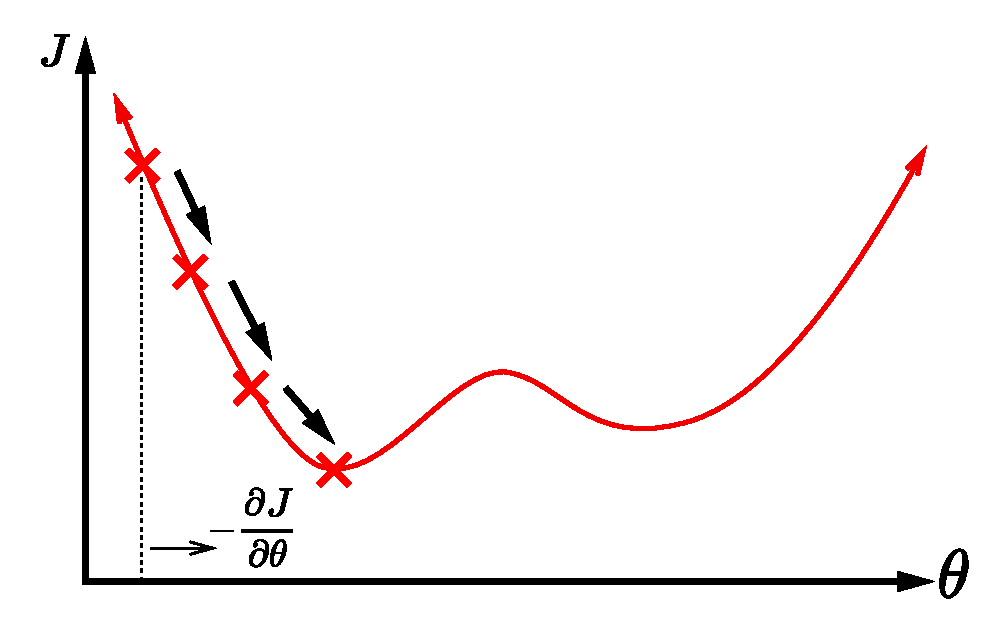
\includegraphics[width=0.5\textwidth]{sketch/gradient_intuition}
%		\caption[]{An illustration of Gradient Descent}
%		\label{fig:gradent_descent_toy}
%	\end{center}
%\end{figure}

\begin{align}
 \forall \theta_i \in \btheta : \theta_i \leftarrow \theta_i - \lambda  \frac{\partial J_{emp} }{\partial \theta_i}
\label{eq:gradient_update}
\end{align}

 Let's 
consider again the NN shown in \addfigure{\ref{fig:nn_typical_structure}} with a loss function $L$ and assume that the network uses activation functions $\sigma$ and has $\btheta = \{ \forall i,j,k,l : w^{(1)}_{ij}, w^{(2)}_{jk}, w^{(3)}_{kl}  \}$ with biases omitted. Given a pair of a sample and its true label $(\x, y)$, the forward pass computations are

\begin{align*}
		h_j^{(1)} &= \sum_i w_{ij}^{(1)} x_i & a_j^{(1)} &= \sigma (h_j^{(1)})	\\
		h_k^{(2)} &= \sum_j w_{jk}^{(2)} a_j^{(1)}  & a_k^{(2)} &= \sigma (h_k^{(2)})	 \\
		h_l^{(3)} &= \sum_k w_{kl}^{(3)} a_k^{(2)} & a_l^{(3)} &= \sigma (h_l^{(3)})	 \\
		f(\x) &= \boldsymbol{a}^{(3)}
\end{align*}

The gradient $\nabla_{\boldsymbol{\theta}} J_{emp}$ can be efficiently computed by backwardly applying the chain rule from the last layer to the first layer. This results in the \textit{backpropagation} algorithm.
\begin{align*}
	\frac{\partial L(f(\x), y)  }{\partial w_{k  l}^{(3)} } &= 	\frac{\partial L(f(\x), y) }{\partial a_{l}^{(3)} }  \frac{\partial a_{l}^{(3)} }{\partial w_{k  l}^{(3)} }  	\\
		&= 	\underbrace{\frac{\partial L(f(\x), y) }{\partial a_{l}^{(3)} } \sigma'(h_l^{(3)})}_{ \delta_l^{(3)}} a_{k}^{(2)} 	\\
	\frac{\partial L(f(\x), y)  }{\partial w_{j  k}^{(2)} } 
		&=  \sum_{l'} 	\frac{\partial L(f(\x), y) }{\partial a_{l'}^{(3)} } \frac{\partial a_{l'}^{(3)}}{\partial w_{j  k}^{(2)}} \\
		&= \sum_{l'} 	\frac{\partial L(f(\x), y) }{\partial a_{l'}^{(3)} } \sigma'(h_{l'}^{(3)})  \frac{\partial h_{l'}^{(3)} }{\partial w_{j  k}^{(2)}} \\
		&= \sum_{l'} 	\delta_{l'}^{(3)}  w_{k  l'}^{(3)} \frac{\partial a_{k}^{(2)} }{\partial w_{j  k}^{(2)}} \\
		&= a_{j}^{(1)}  \underbrace{\sigma'(h_{k}^{(2)}) \sum_{l'}\delta_{l'}^{(3)} w_{k  l'}^{(3)}}_{\delta_{k}^{(2)}}  \\
	\frac{\partial L(f(\x), y)  }{\partial w_{i  j}^{(1)} } &=  x_i  \sigma'(h_{j}^{(1)}) \sum_{k'} 	\delta_{k'}^{(2)} w_{j  k'}^{(2)} 
\end{align*}

As shown in the derivations above, computing the gradient backward allows us to reuse previously calculated quantities, such as $\delta_l^{(3)}, \delta_{k}^{(2)}$, hence saving computational resources.  It is worth noting that these  quantities can be interpreted as amount of error propagated to responsible neurons in the network.

%
%As shown in the derivations above, backpropagation allows us to efficiently compute the gradients by reusing previously calculated gradients from the later layer, for example $\delta_l^{(3)}, 	\delta_{k}^{(2)}$. Moreover, these reused quantities can be also interpreted as error propagated to responsible neurons.

In practice, because the training set $D$ usually contains several thousand samples, an execution of  (\ref{eq:gradient_update}) would require significant amount of memory to store necessary calculations. Therefore, the training data $D$ is equally divided into mini batches  $\widetilde{D}_i$  and a gradient update is  performed for every $\widetilde{D}_i$. Practically,  the size of $\widetilde{D}_i$ is chosen between 32 and 512 samples. This is referred to as the \textit{mini-batch gradient descent} approach.




%Lastly, because noise in training data and potentially highly non-smooth of the cost function, learning rate $\lambda$ has great influential on the training process. More precisely, it should not be too small or too large. This requires some effort and experience in order to get the value right. Some work have proposed alternative update rules aiming to make the training process more stable. For example,  \textit{Adaptive Moment Estimation}(Adam)\citep{KingmaAdamMethodStochastic2014}  uses an adaptive learning rate  and incorporates accumulated direction and speed of the previous gradients(\textit{momentum}) into the adjustment, hence more consistent gradient and fast convergence. Other similar proposals are RMSProp\citep{TielemanLectureRmsPropDivide2012} and Adadelta\citep{ZeilerADADELTAAdaptiveLearning2012}.


%
%\subsection{Convolutional Neural Networks} \label{sec:conv}
%Convolutional neural networks(CNN) refer to neural networks that employ convolutional operators to process input instead of fully-connected layers(weighted sum). Typically, a convolutional operator is followed by a pooling operator. Using this convolutional and pooling operators allows the neural network to extract hierarchical features that are spatially invariant \cite{ZeilerVisualizingUnderstandingConvolutional2013}. Hence, these type of layers increases predictive capability of NN, while using fewer parameters than traditional fully-connected layers.
%
%%\afterpage{
%\begin{figure}[!hbt]
%    \begin{center}
%		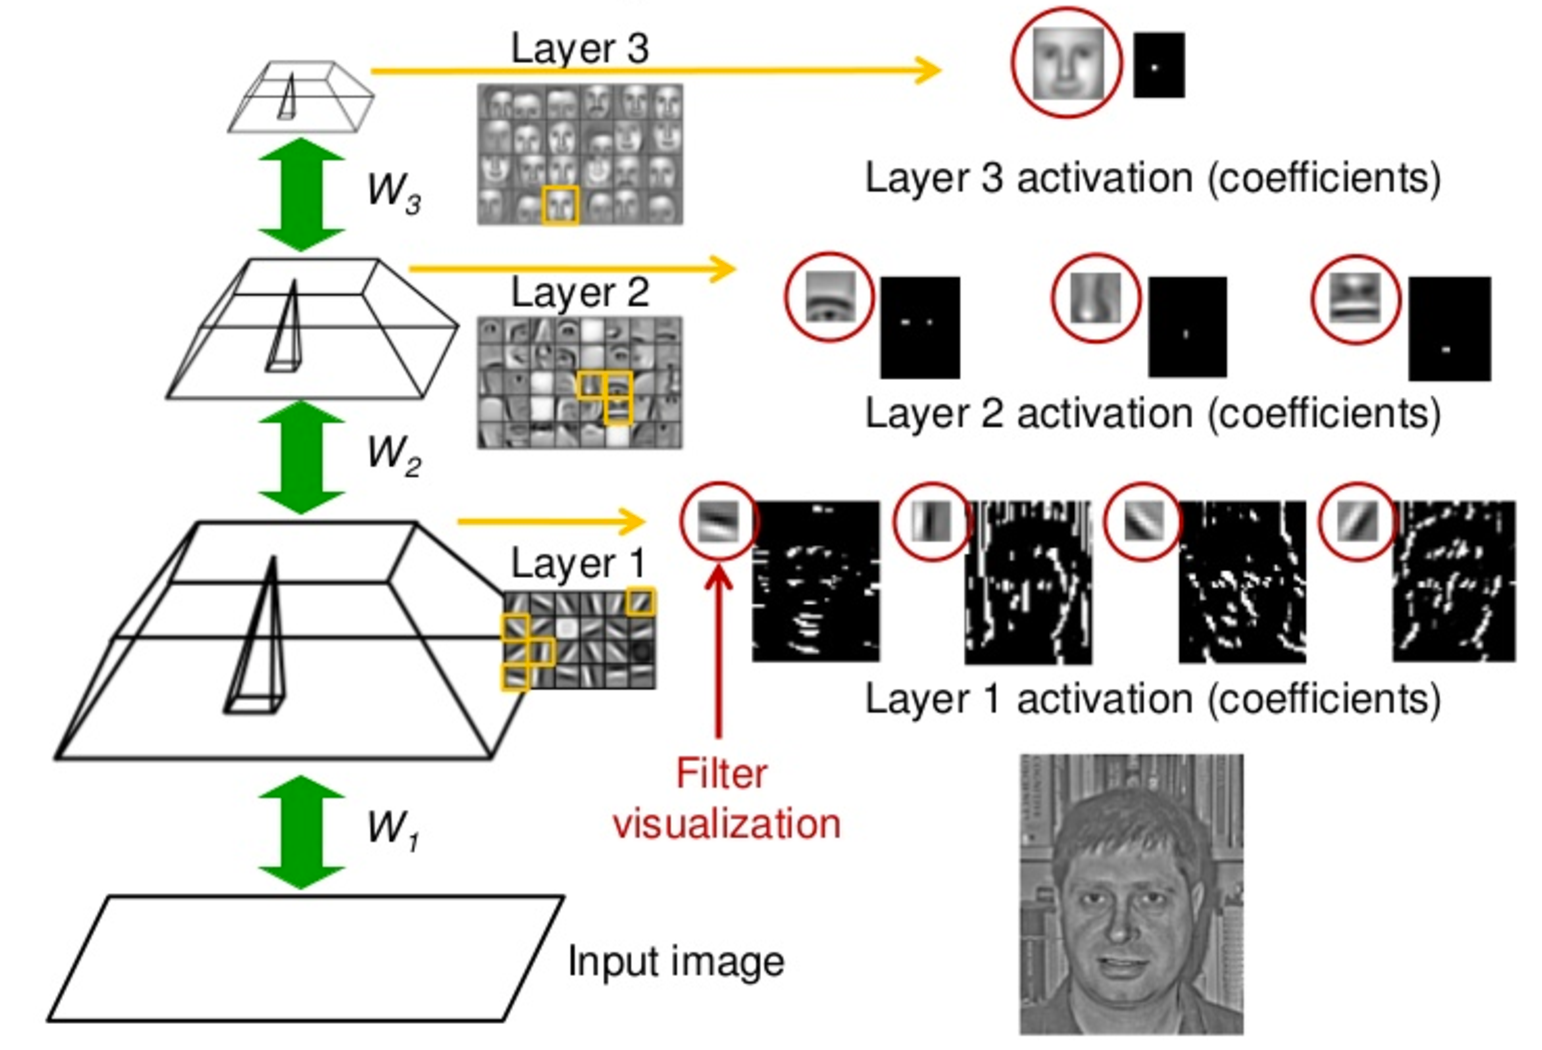
\includegraphics[width=0.5\textwidth]{sketch/cnn_hierachical_features}
%		\caption{Hierarchical features learned by a CNN.}
%		\label{fig:conv_intuition}
%		\small{Source : \cite{LeeConvolutionalDeepBelief2009}}
%	\end{center}
%\end{figure}
%
%
%\addfigure{\ref{fig:conv_intuition}} illustrates hierarchical structures that neurons in each layer of a CNN learn to detect. More precisely, this example shows that neurons in the first learn to detect low level features, such as edges, and neurons in middle layer then use knowledge to detect higher level features, for example, nose, mouth or eyes.
%
%
%%\afterpage{
%\begin{figure}[!hbt]
%    \begin{center}
%		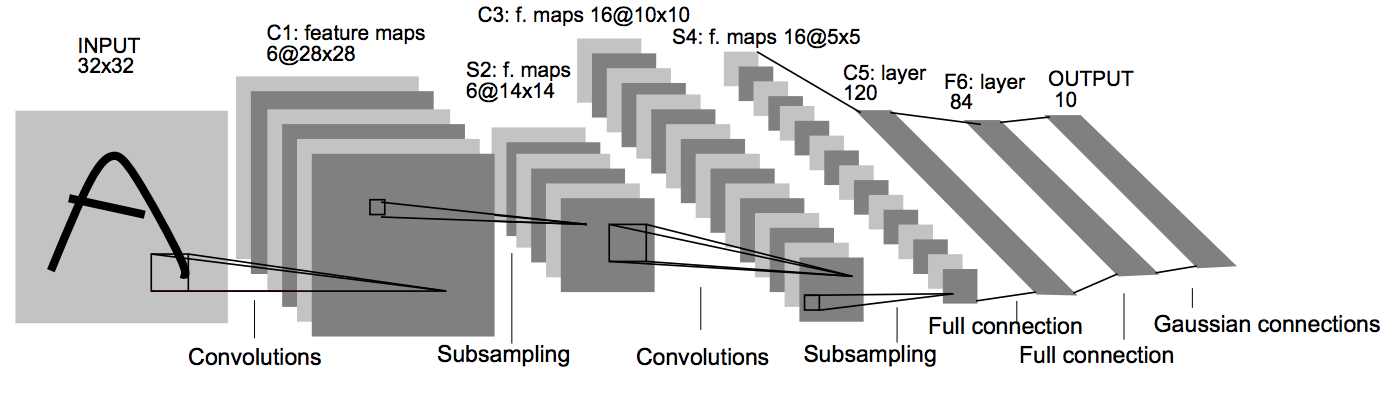
\includegraphics[width=0.8\textwidth]{lenet}
%		\caption{LeNet-5 architecture for a digits recognition task.}
%		\label{fig:lenet}
%		\small{ Source : \cite{LeCunGradientBasedLearningApplied2001} }
%	\end{center}
%\end{figure}
%
%
%Since \cite{LeCunGradientBasedLearningApplied2001} proposed LeNet-5, shown in \addfigure{\ref{fig:lenet}}, and successfully applied it to handwritten recognition problems, CNN have become the first choice of architectures in many domains. Particularly, in computer vision, CNN are the major component of state-of-the-art results in various contests. Such successful results are :  AlexNet\citep{KrizhevskyImageNetClassificationDeep2012} that archive  remarkable results on  ImageNet Large-Scale Visual Recognition Challenge 2012(ILSVRC 2012) followed by the achievement of VGG\citep{SimonyanVeryDeepConvolutional2014} and GoogleLenet \citep{SzegedyGoingdeeperconvolutions2015} architecture in ILSVRC 2014 and ResNet\citep{HeDeepResidualLearning2016} in ILSVRC 2015.
%
%

\section{Recurrent Neural Networks}
Unlike typical neural networks (feedforward architectures), recurrent neural networks (RNNs) are a type of neural networks whose outputs are repeatedly incorporated back into next computations of the network. Having a recurrent mechanism allows RNNs to build suitable representations (\textit{states}) to solve problems dealing with sequential data,  such as machine translation and natural language processing (NLP).

\subsection{Unfolding a RNN and Backpropagation Through Time}
 
\addfigure{\ref{fig:rnn_unfold}} illustrates the general setting of a RNN and its unfolded computational graph. Let's consider a sequence $\x= \{ x_t \}_{t=1}^{T}$ and $r_0 = 0$.  At step $t$, the RNN takes  the corresponding input $x_{t}$ and the previous recurrent state $r_{t-1}$ to compute the new recurrent state $r_{t}$ and the output $\hat{y}_t$. For problems, such as classification, that we are only interested the prediction at the last step $t=T$, $\{ \hat{y}_t \}_{t=1}^{T-1}$ can be omitted. Let's assume that it is the case here and $w_x$ and $w_r$ are parameters of the network.  The forward pass is then

\begin{align*}
	h_1 &= w_{x} x_1 + w_{r} r_0 & r_1 &= \sigma(h_1)  \\
	h_2 &= w_{x} x_2 + w_{r} r_1 &  r_2 &= \sigma(h_2) \\
	& \vdots & \vdots \\
	h_{T} &= w_{x} x_{T} + w_{r} r_{T-1} &  r_{T} &= \sigma(h_{T}) \\
	\hat{y}_T &= r_T
\end{align*}
By unfolding the network,  we can see that RNNs are a special case of feedforward architectures where layers share the same parameters. Hence, RNNs can be trained by the backpropagation algorithm and their predictions can also be interpreted by the explanation techniques developed for feedforward architectures.


\begin{figure}
\centering
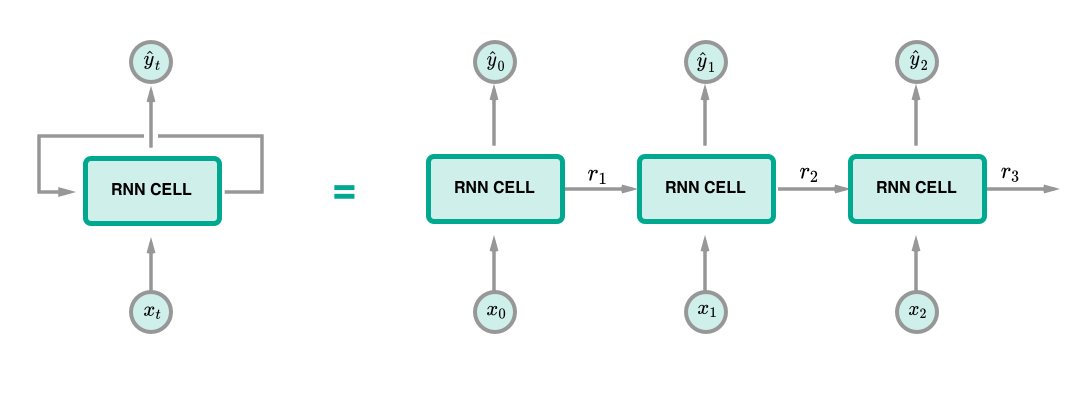
\includegraphics[width=\textwidth]{sketch/rnn_unfold}
\patcaption{The unfolded computational graph of a RNN  transforming an input sequence $\{ x_t \}_{t=1}^{T}$ to a corresponding output sequence $\{ \hat{y}_t \}_{t=1}^T$.}{Adapted from \citep{OlahUnderstandingLSTMNetworks2015}.}
\label{fig:rnn_unfold} 
\end{figure}

Because weights in RNNs are shared between layers used at  each time step, the gradient needs to be backpropagated from every corresponding computation step. This is referred to as \textit{backpropagation through time} (BPTT). For \addfigure{\ref{fig:rnn_unfold}}, the gradient can be calculated as follows:

\begin{align*}
	\patpartial{L(f(\x), y)}{w_x} &= \sum_{t=1} ^{T} 	\patpartial{L(f(\x), y)}{r_T} \patpartial{r_T}{r_t} \frac{\partial_+r_t}{ \partial w_x} \\ 
				&= \sum_{t=1} ^{T} 	\patpartial{L(f(\x), y)}{r_T} \patpartial{r_T}{r_t} \sigma'(h_t)x_t \\
				&= \sum_{t=1} ^{T} 	\patpartial{L(f(\x), y)}{r_T} \sigma'(h_t)x_t \Bigg( \prod_{T \ge i > t} \patpartial{r_i}{r_{i-1}} \Bigg) \\
				&= \sum_{t=1} ^{T} 	\patpartial{L(f(\x), y)}{r_T} \sigma'(h_t)x_t \Bigg( \prod_{T \ge i > t} w_r \sigma'(h_i) \Bigg) \\
				&= \sum_{t=1} ^{T} 	\patpartial{L(f(\x), y)}{r_T}  x_t \Bigg( w_r^{T-t} \Bigg) \Bigg( \prod_{T \ge i \ge t} \sigma'(h_i) \Bigg) \\
\frac{\partial L(f(\x), y)}{\partial w_{r}} &=  \sum_{t=1} ^{T} 	\patpartial{L(f(\x), y)}{r_T} \patpartial{r_T}{r_t} \frac{\partial_+r_t}{ \partial w_r} \\
				&= \sum_{t=1} ^{T} 	\patpartial{L(f(\x), y)}{r_T}  r_{t-1} \Bigg( w_r^{T-t} \Bigg) \Bigg( \prod_{T \ge i \ge t} \sigma'(h_i) \Bigg),
\end{align*}
where $\frac{\partial_+r_t}{ \partial w_x}$ and  $\frac{\partial_+r_t}{ \partial w_r}$ are the \textit{immediate} partial derivatives  of the recurrent state $r_t$ with respect to $w_x$ and $w_r$, where $r_{t-1}$ is treated as a constant with respect to the weights \citep{Pascanudifficultytrainingrecurrent2013}.

Although RNNs can model sequences with any length, the length of training sequences is typically fixed before applying BPTT. This makes the implementation more straightforward and also allows memory usage during the training to be controlled. However, RNNs still need to be trained on long-enough sequences to learn long-term dependencies properly. As can be seen from the derivations above, this requirement can negatively impact the learning efficiency. In particular, \citet{BengioLearninglongtermdependencies1994} and \citet{ Pascanudifficultytrainingrecurrent2013} analytically discussed two potential problems that might happen to the gradient, namely

%
%improves learning efficiency. dd
%As the number of computation steps in RNN is depend on the length of samples, which can be different in principle, one needs to organize data in such a way that samples in the same batch have the same  length of computation before training a RNN. As a result, training RNNs can be viewed as training a feedforward neural network with a certain depth of layers, hence backpropagation can be readily applied. In this case, the difference between NN and RNN is the fact that variables are shared the same across layers.
%
%
%%
%However, as the computations unfolded, we can see that there are 2 problems that might happen to the gradients of the shared parameters $w_{rx}$ and $ w_{rr}$, namely
\begin{itemize}
   %todo unclear exploding gradient
	\item \textit{Exploding gradient} happens when the spectral radius of the recurrent weight matrix is greater than 1. This radius is the largest of absolute eigenvalues of the matrix. In this example, the radius is simply $|w_r|$\footnote{A scalar value can be viewed as a $1 \times 1$ matrix; hence the largest eigenvalue is the element itself.}. As can be seen from the derivations above, when $|w_r|$ is larger than 1, the exponential term will quickly result in a gradient with a considerable large norm leading to an unreliable training. \citet{Pascanudifficultytrainingrecurrent2013} proposed the \textit{gradient clipping} technique to alleviate the problem.
	\item \textit{Varnishing gradient} in contrast occurs when the radius is smaller than one. This yields a gradient with near-zero norm. This issue leads to slow learning; hence RNN would require enormous amount of time to learn long-term dependencies. The next section discusses approaches proposed to mitigate this problem.
\end{itemize}



\subsection{Long Short-Term Memory and Gated RNNs}
The varnishing gradient is a crucial problem that causes RNNs to learn long-term memories with a slow progress. The issue is primarily due to  how the computation of the recurrent state  is constructed. In particular, as described previously, standard RNNs compute the state through a weighted sum at every step $t$ leading to the exponential term of the recurrent weights in the computation of the gradient.

Alternatively, \citet{HochreiterLongshorttermmemory1997} proposed the \textit{Long Short-Term Memory} architecture (LSTM) that employs gating mechanisms and an additive update in the computation of the recurrent state. Using this approach  decreases the number of potential damping terms involved in the gradient computation, hence LSTM can learn long term dependencies much more efficiently than standard RNNs. It should be noted that LSTM still suffers from the exploding gradient problem.

As shown in \addfigure{\ref{fig:lstm_structure}}, LSTM utilizes three gates, namely input $i_g$, forget $f_g$ and output $o_g$ gates controlling information flow through the network. More precisely, the $f_g$ gate decides how much the information from the previous cell state $C_{t-1}$ is kept, while the $i_g$ gate decides the amount of information from the previous output $h_{t-1}$ and the current input $x_t$ will be considered.  The combination of the results from these two gates is the new cell state $C_{t}$. On the other hand, the $o_g$ gate determines the output information $h_t$ leaking from the current cell state $C_t$. Mathematically, 
\begin{align*}
	i_g &= \sigmoid( w_{ix} x_t + w_{ih} h_{t-1} )  &  	f_g &= \sigmoid( w_{fx} x_t + w_{fh} h_{t-1} )\\
	o_g &= \sigmoid( w_{ox} x_t + w_{oh} h_{t-1} ) & \widetilde{C}_t &= \tanh(w_{cx} x_t + w_{ch} h_t) \\
	C_t &= f_g \otimes C_{t-1} + i_g  \otimes  \widetilde{C}_t & h_{t} &= o_g \otimes \tanh(C_t),
\end{align*}

where $\otimes$ the element-wise multiplication.


\begin{figure}
\centering
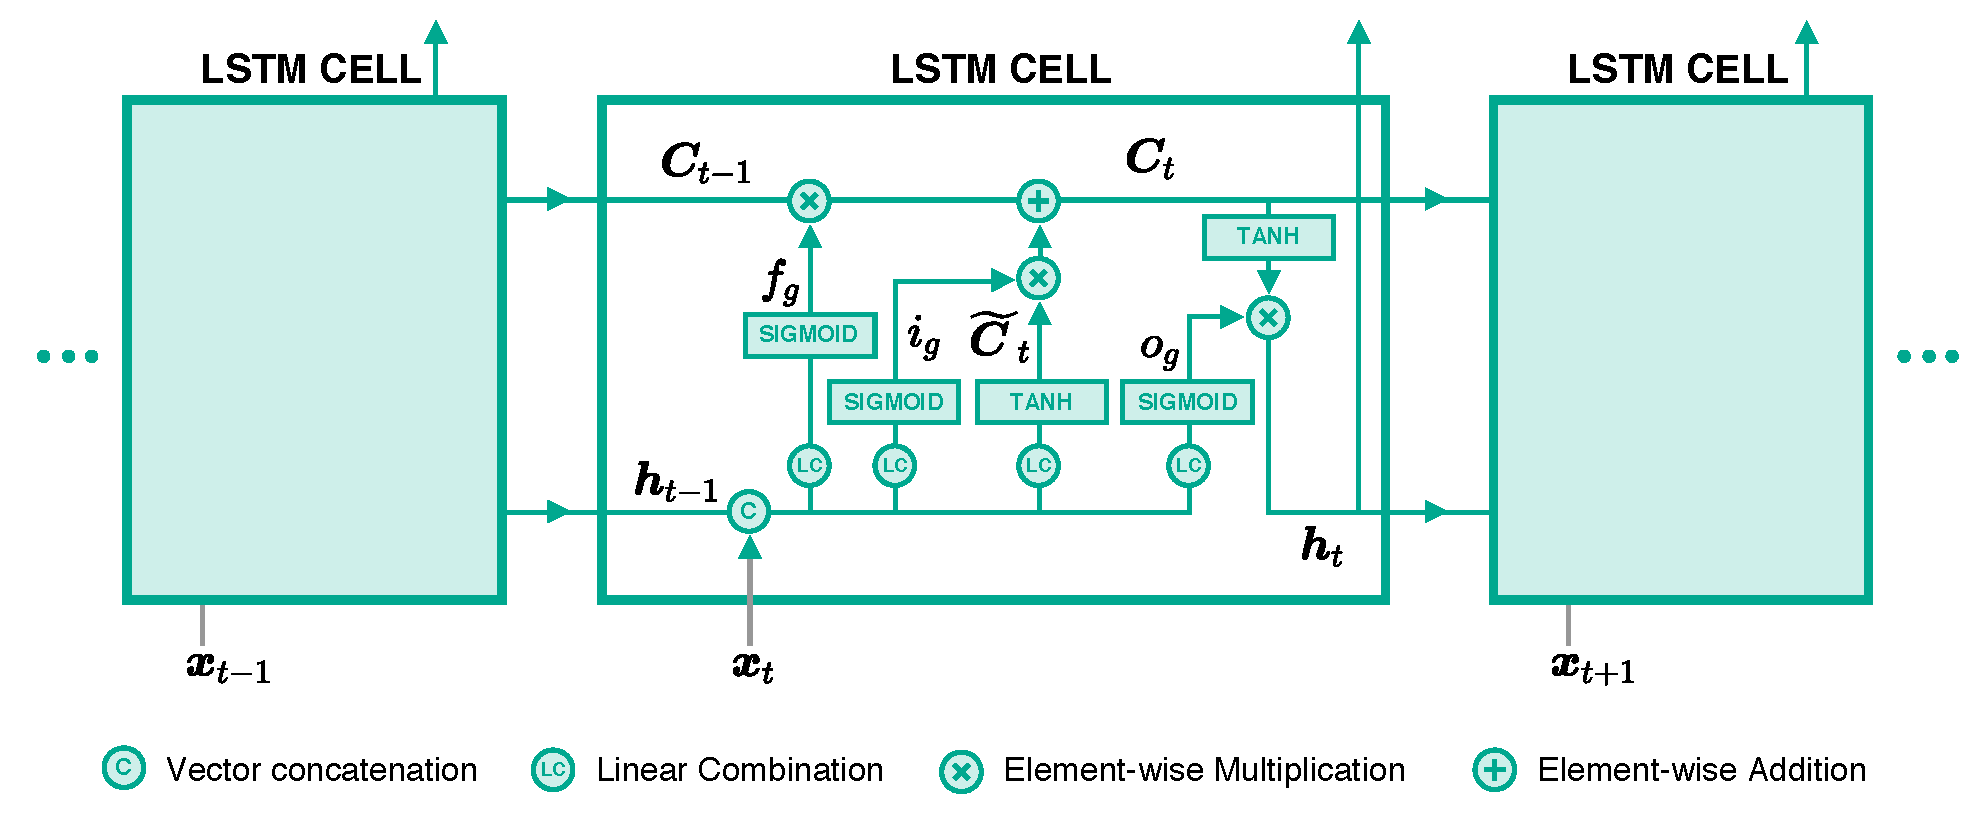
\includegraphics[width=1\textwidth]{sketch/lstm}
\patcaption{LSTM structure.}{Adapted from \citep{OlahUnderstandingLSTMNetworks2015}.}

\label{fig:lstm_structure} 
\end{figure}

Despite the fact that  LSTM has become a core component of many state-of-the-art sequence modeling applications, such as machine translation \citep{MelisStateArtEvaluation2018}, it is still obscure whether we need that many gates in the LSTM. In particular, \citet{GreffLSTMsearchspace2017} demonstrated that the forget and output gates are the crucial parts of the LSTM.  \citet{ChoLearningPhraseRepresentations2014a} proposed the \textit{Gated Recurrent Unit} architecture (GRU) that employs only two	 gates; however, \citet{JozefowiczEmpiricalExplorationRecurrent2015} conducted several benchmarking tasks and found no significant difference in performance between LSTM and GRU. 

% todo
%- viable length
%- output each step is not necessary
%- summarize input
%- type od RNN
% - seq2seq, seq2vector...
